\documentclass[12pt,a4paper]{report}
\usepackage[margin=1in]{geometry}
\usepackage{graphicx}
\usepackage{float}
\usepackage{subcaption}
\usepackage{hyperref}
\usepackage{fancyhdr}

\pagestyle{fancy}
\fancyhf{}
\rhead{Memory Allocation Using Segmentation}
\lhead{Spring 2026}
\cfoot{\thepage}

\title{\textbf{Memory Allocation Using Segmentation}}
\author{}
\date{\today}

\begin{document}

\maketitle

\section*{Brief Explanation}
This project demonstrates memory allocation using segmentation with two strategies: First-Fit and Best-Fit. The GUI shows the memory layout, the segment table, and the free holes after each operation.

\section*{Simple Code Explanation}
The code is split into a few main parts:
\begin{itemize}
    \item \textbf{MemoryManager}: this is the part that does the real work. It keeps track of free holes and decides where each process will go.
    \item \textbf{Process, Segment, and Hole}: these are small data models. They store the name, size, and address of each process part or free space.
    \item \textbf{MainWindow}: this controls the GUI. It connects the buttons, tables, and memory view to the allocation logic.
    \item \textbf{MemoryCanvas}: this draws the memory blocks on the screen so the user can see what is allocated and what is free.
    \item \textbf{main\_window.ui and styles.qss}: these files define the interface layout and the visual style.
\end{itemize}

In short, the program starts with free holes, then it places each process into memory using First-Fit or Best-Fit. After each step, the GUI updates the tables and the memory drawing so the result is easy to follow.

\section*{Important Code Snippets}
\subsection*{1. Memory allocation}
This part tries to place every segment of a process into memory.
\begin{verbatim}
def allocate_process(self, process, method):
    working_holes = [Hole(hole.start, hole.size) for hole in self.holes]
    for segment in process.segments:
        hole_index = self._find_hole_index(working_holes, segment.size, method)
        if hole_index is None:
            process.allocated = False
            return False
        hole = working_holes[hole_index]
        segment.start = hole.start
        hole.start += segment.size
        hole.size -= segment.size
    self.holes = sorted(working_holes, key=lambda hole: hole.start)
    process.allocated = True
    return True
\end{verbatim}

\subsection*{2. Choosing the hole}
This part decides where to put the next segment.
\begin{verbatim}
def _find_hole_index(holes, size, method):
    if method == AllocationMethod.FIRST_FIT:
        for index, hole in enumerate(holes):
            if hole.size >= size:
                return index
        return None

    best_index = None
    best_waste = None
    for index, hole in enumerate(holes):
        if hole.size >= size:
            waste = hole.size - size
            if best_waste is None or waste < best_waste:
                best_index = index
                best_waste = waste
    return best_index
\end{verbatim}

\subsection*{3. Running the test case}
This part runs the same steps shown in the screenshots.
\begin{verbatim}
steps = [
    ("allocate", "P1"),
    ("allocate", "P2"),
    ("allocate", "P3"),
    ("deallocate", "P1"),
    ("allocate", "P4"),
]
\end{verbatim}

\section*{Test Case}
\begin{itemize}
    \item Total memory: 1000 K
    \item Initial holes: $[0,300]$, $[400,650]$, $[700,900]$
    \item Operations: allocate P1, allocate P2, allocate P3, deallocate P1, allocate P4
    \item The scenario is run once with First-Fit and once with Best-Fit
\end{itemize}

\section*{Screenshots}

\section*{First-Fit}
\begin{figure}[H]
    \centering
    \begin{subfigure}[t]{0.48\textwidth}
        \centering
        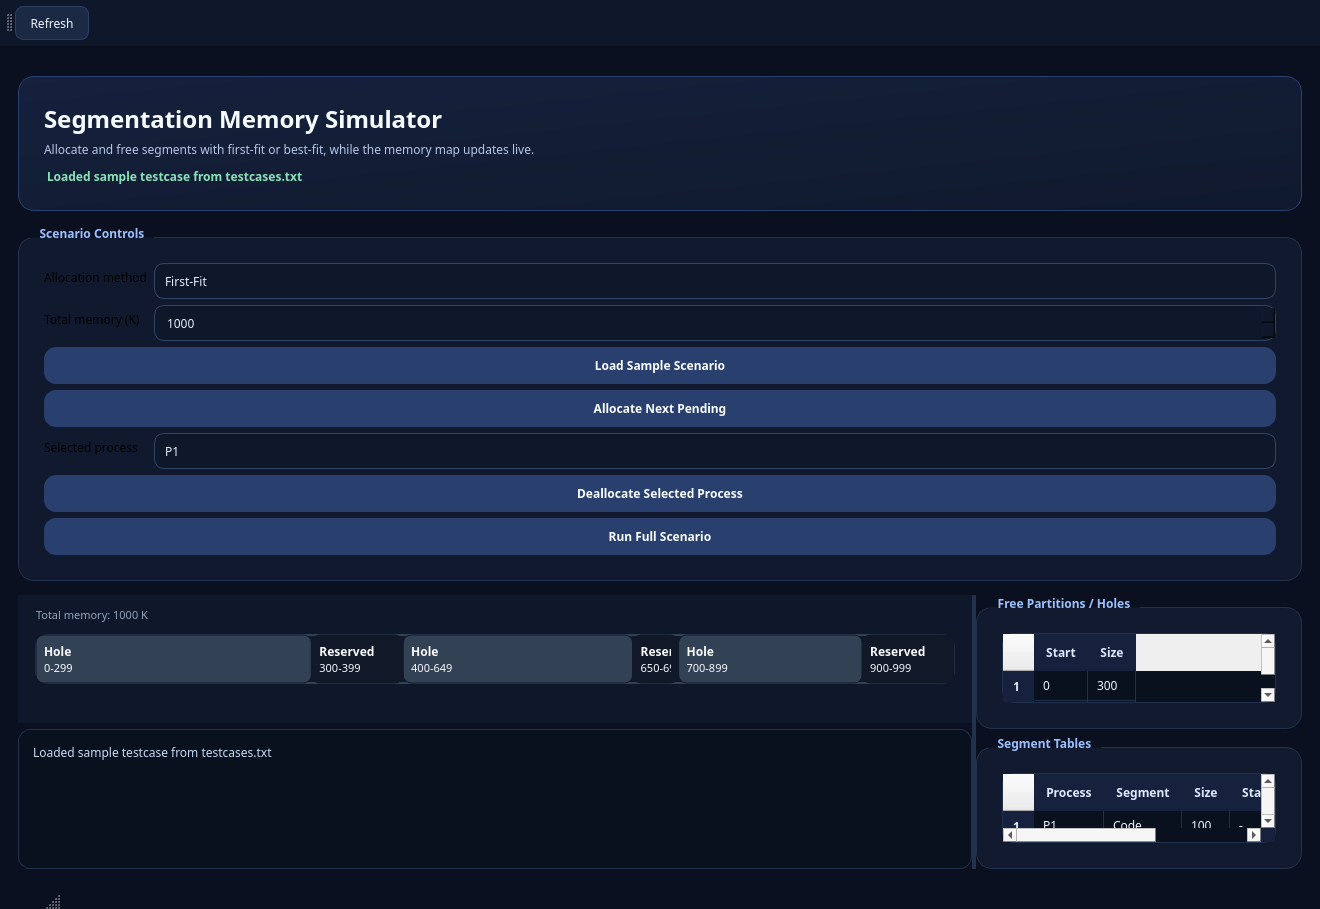
\includegraphics[width=\linewidth]{screenshots/firstfit/initial.png}
        \caption{Initial}
    \end{subfigure}
    \hfill
    \begin{subfigure}[t]{0.48\textwidth}
        \centering
        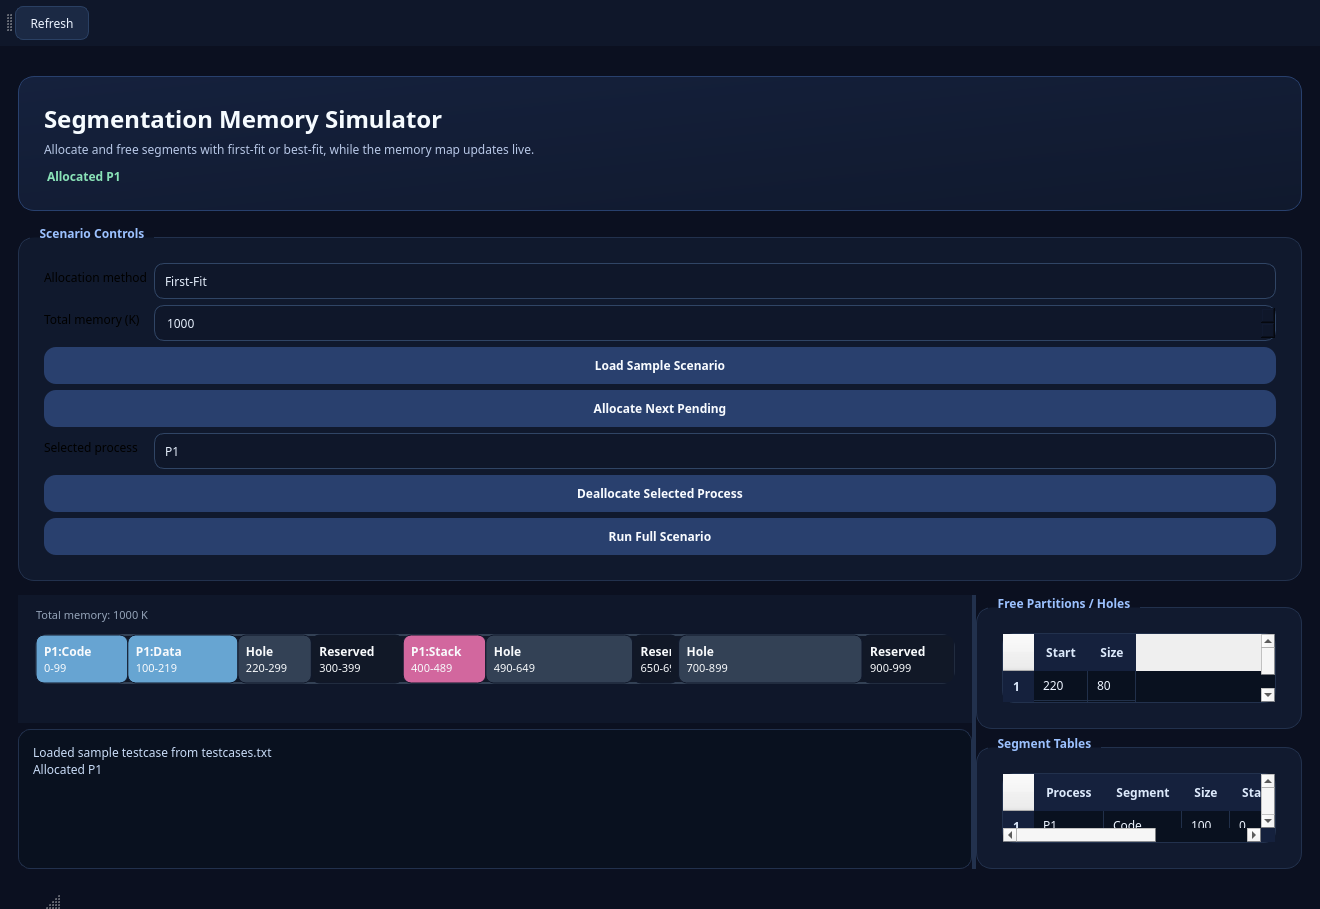
\includegraphics[width=\linewidth]{screenshots/firstfit/p1_allocated.png}
        \caption{P1 allocated}
    \end{subfigure}

    \vspace{0.5cm}

    \begin{subfigure}[t]{0.48\textwidth}
        \centering
        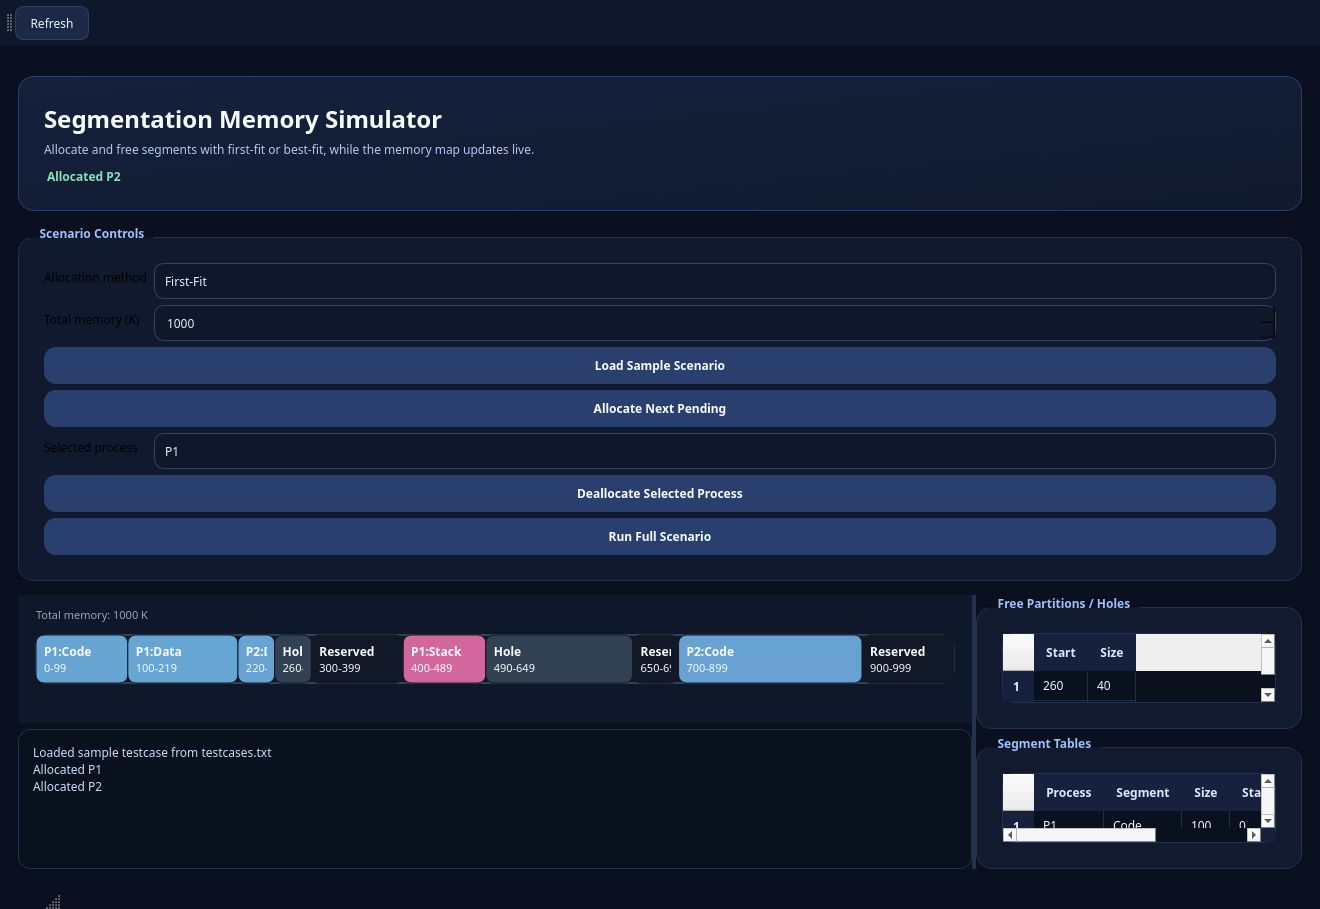
\includegraphics[width=\linewidth]{screenshots/firstfit/p2_allocated.png}
        \caption{P2 allocated}
    \end{subfigure}
    \hfill
    \begin{subfigure}[t]{0.48\textwidth}
        \centering
        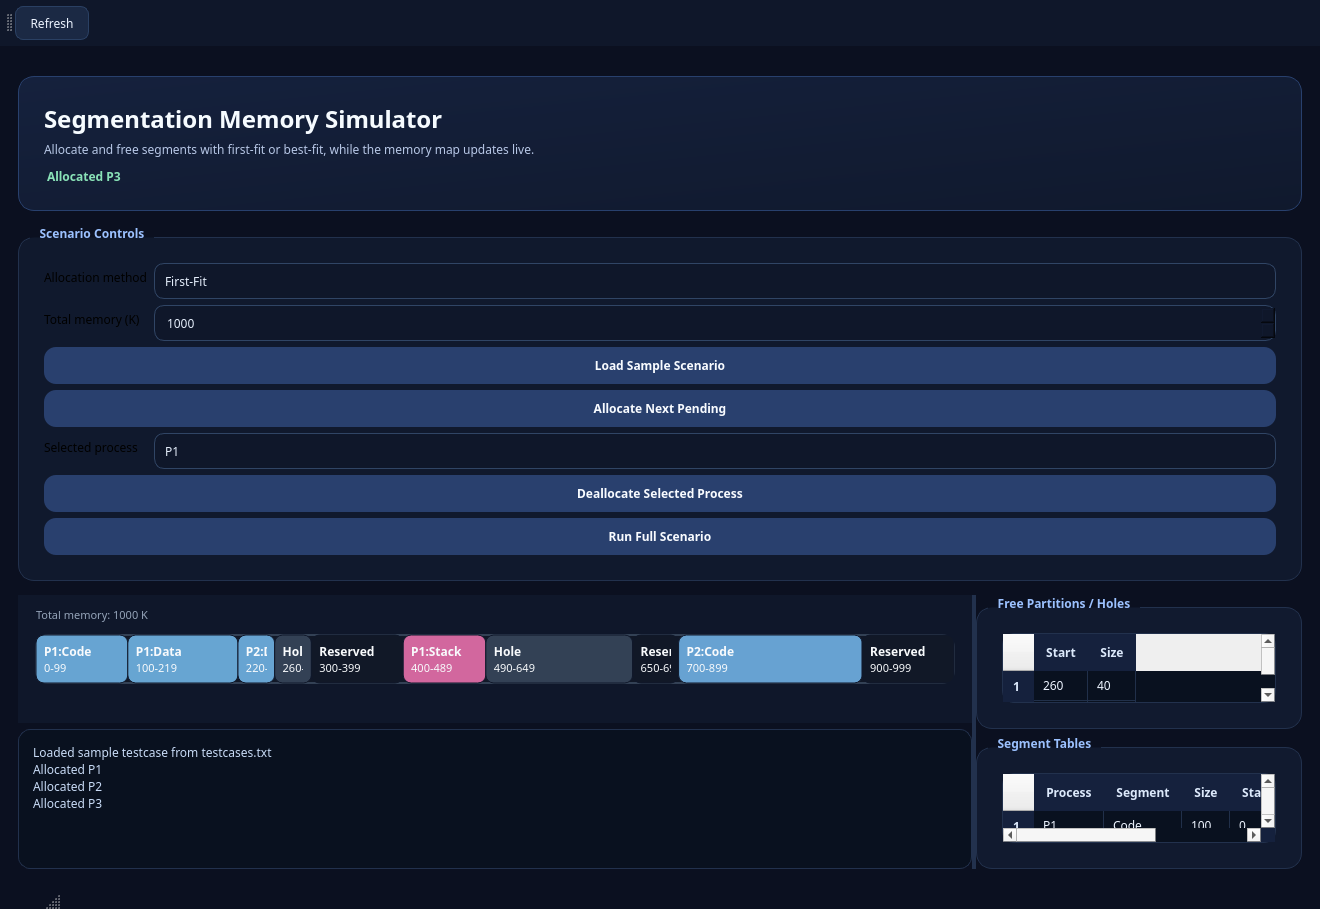
\includegraphics[width=\linewidth]{screenshots/firstfit/p3_attempted.png}
        \caption{P3 attempted}
    \end{subfigure}

    \vspace{0.5cm}

    \begin{subfigure}[t]{0.48\textwidth}
        \centering
        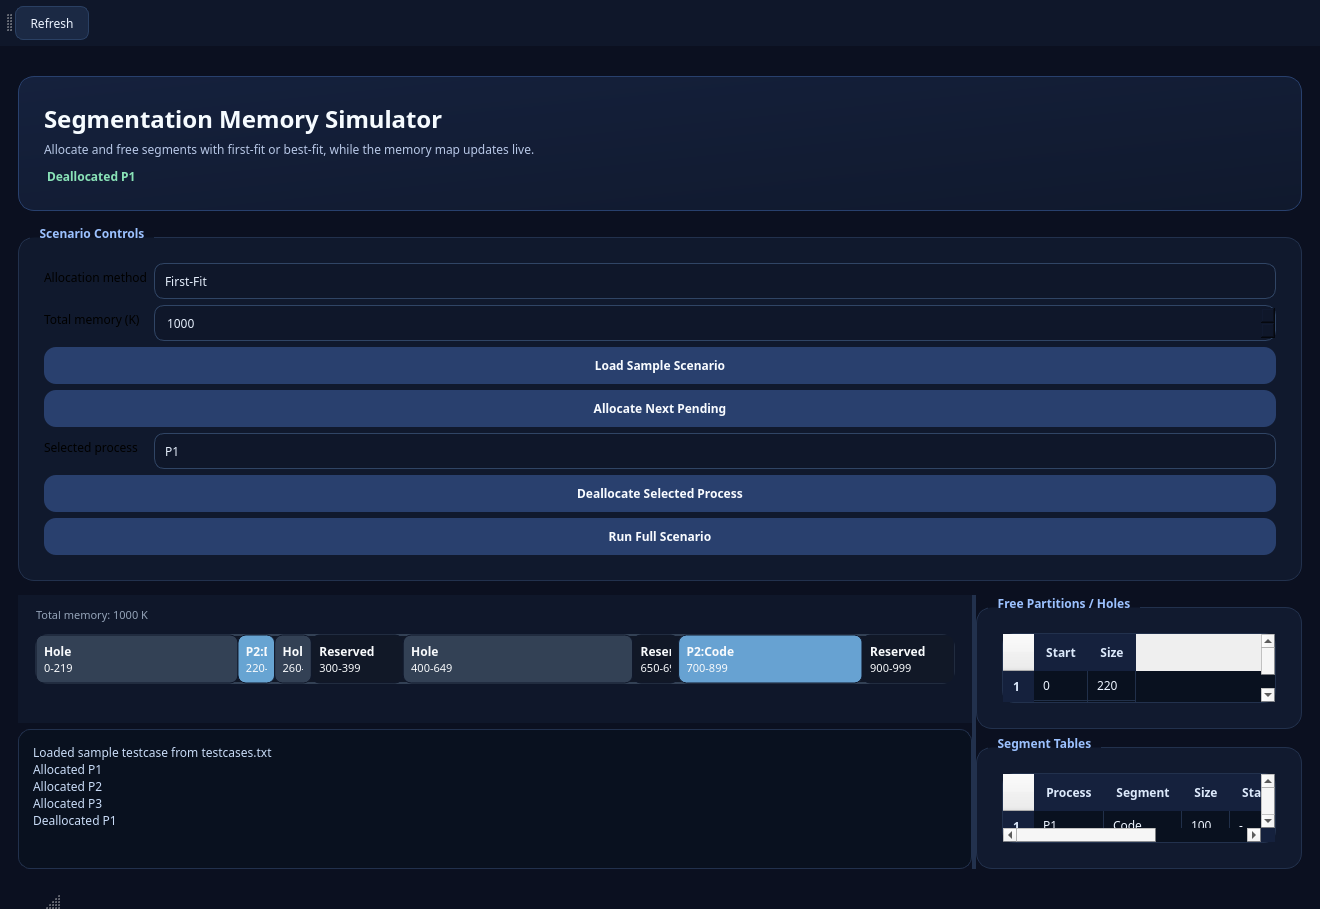
\includegraphics[width=\linewidth]{screenshots/firstfit/p1_deallocated.png}
        \caption{P1 deallocated}
    \end{subfigure}
    \hfill
    \begin{subfigure}[t]{0.48\textwidth}
        \centering
        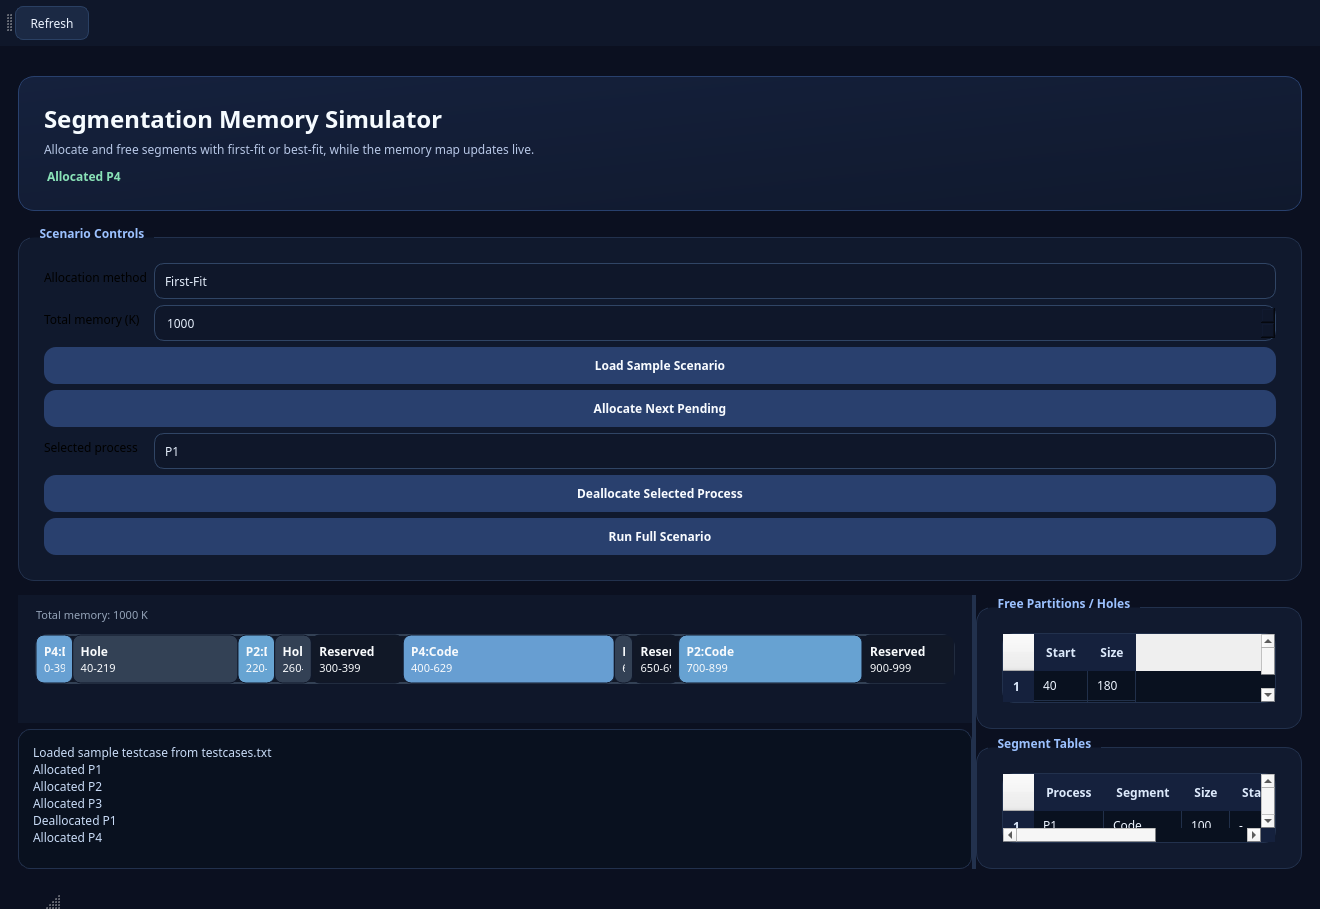
\includegraphics[width=\linewidth]{screenshots/firstfit/p4_allocated.png}
        \caption{P4 allocated}
    \end{subfigure}
    \caption{First-Fit screenshots after each operation.}
\end{figure}

\section*{Best-Fit}
\begin{figure}[H]
    \centering
    \begin{subfigure}[t]{0.48\textwidth}
        \centering
        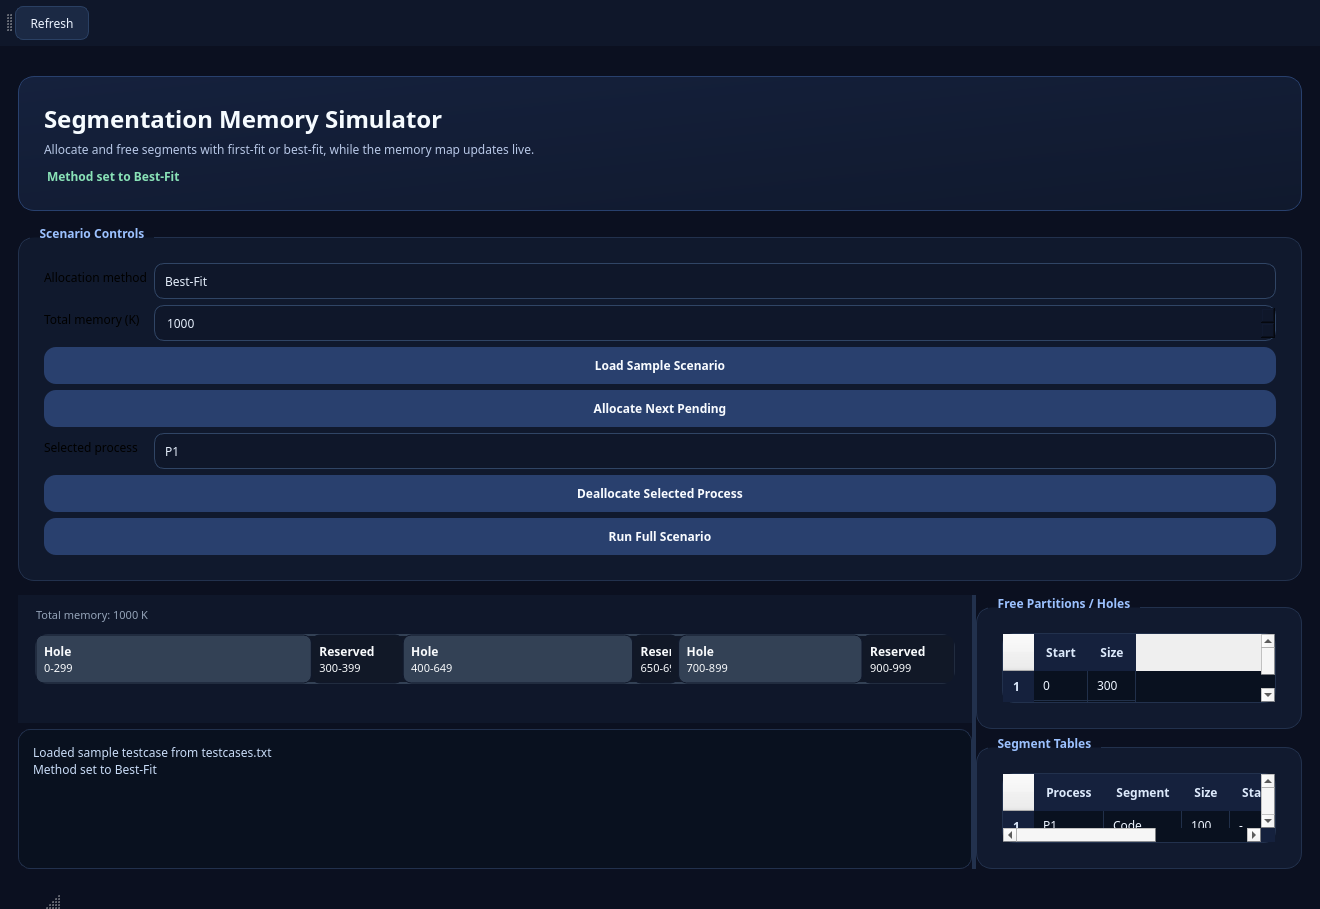
\includegraphics[width=\linewidth]{screenshots/bestfit/initial.png}
        \caption{Initial}
    \end{subfigure}
    \hfill
    \begin{subfigure}[t]{0.48\textwidth}
        \centering
        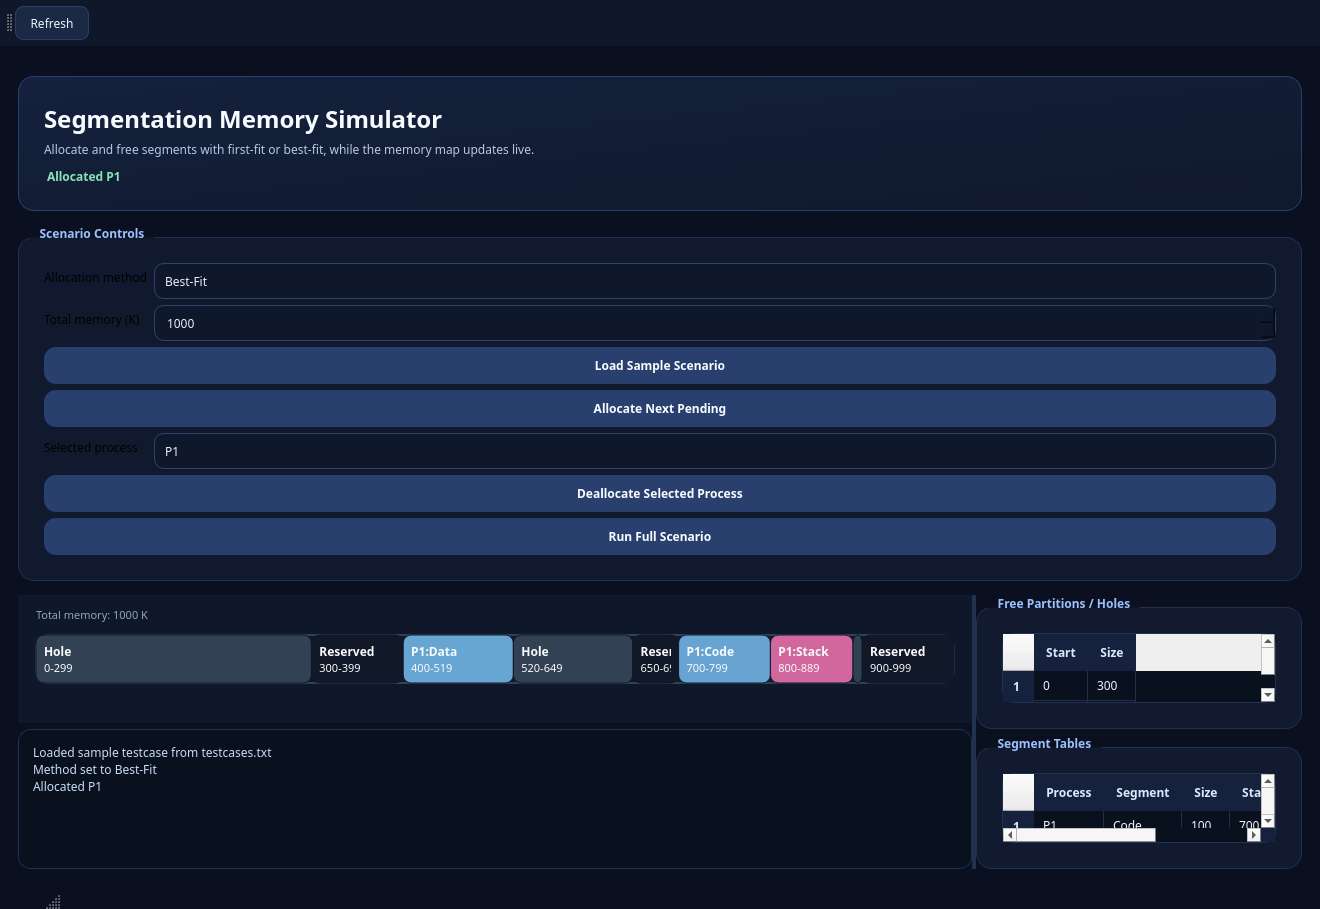
\includegraphics[width=\linewidth]{screenshots/bestfit/p1_allocated.png}
        \caption{P1 allocated}
    \end{subfigure}

    \vspace{0.5cm}

    \begin{subfigure}[t]{0.48\textwidth}
        \centering
        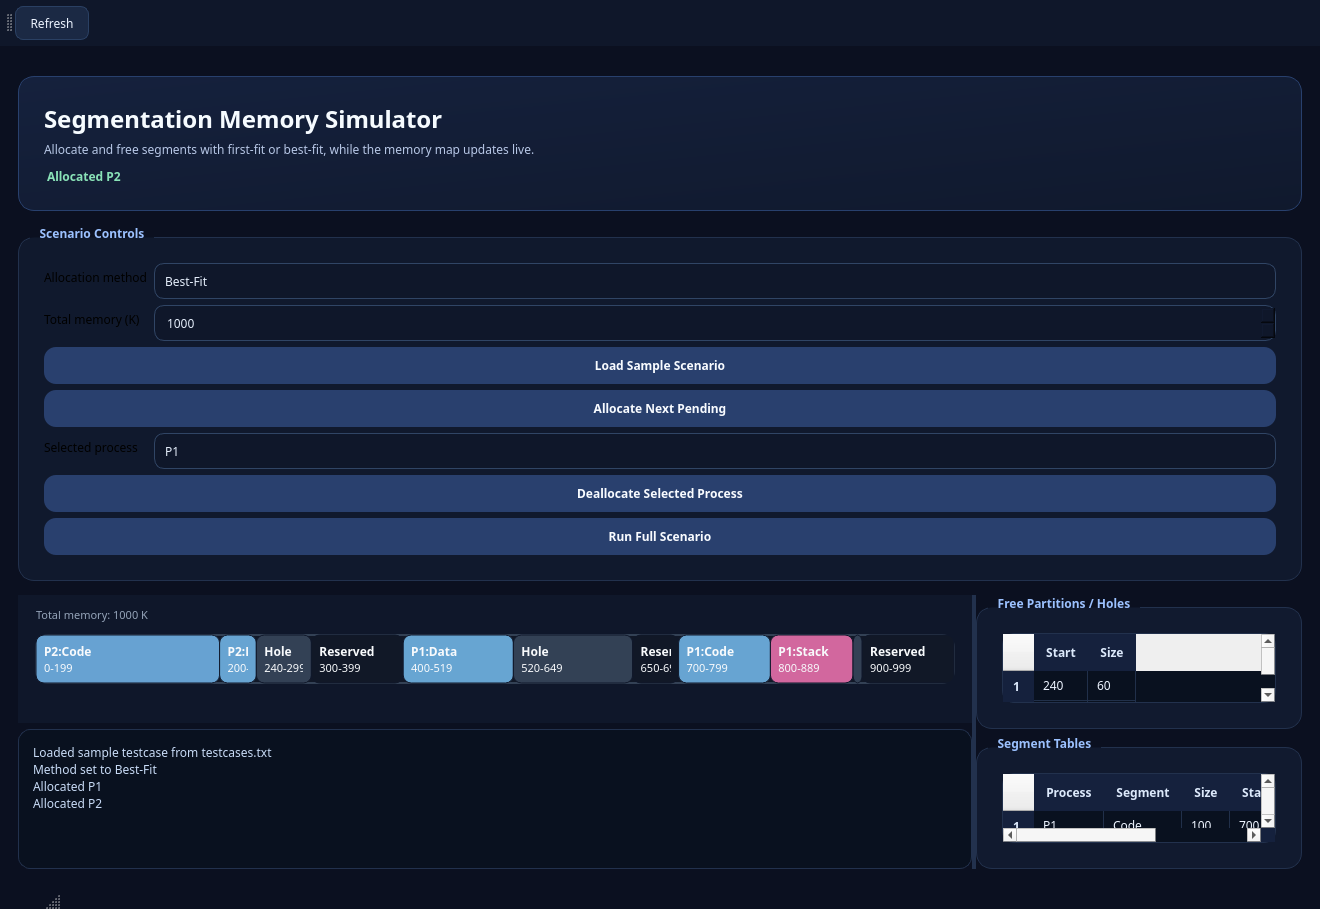
\includegraphics[width=\linewidth]{screenshots/bestfit/p2_allocated.png}
        \caption{P2 allocated}
    \end{subfigure}
    \hfill
    \begin{subfigure}[t]{0.48\textwidth}
        \centering
        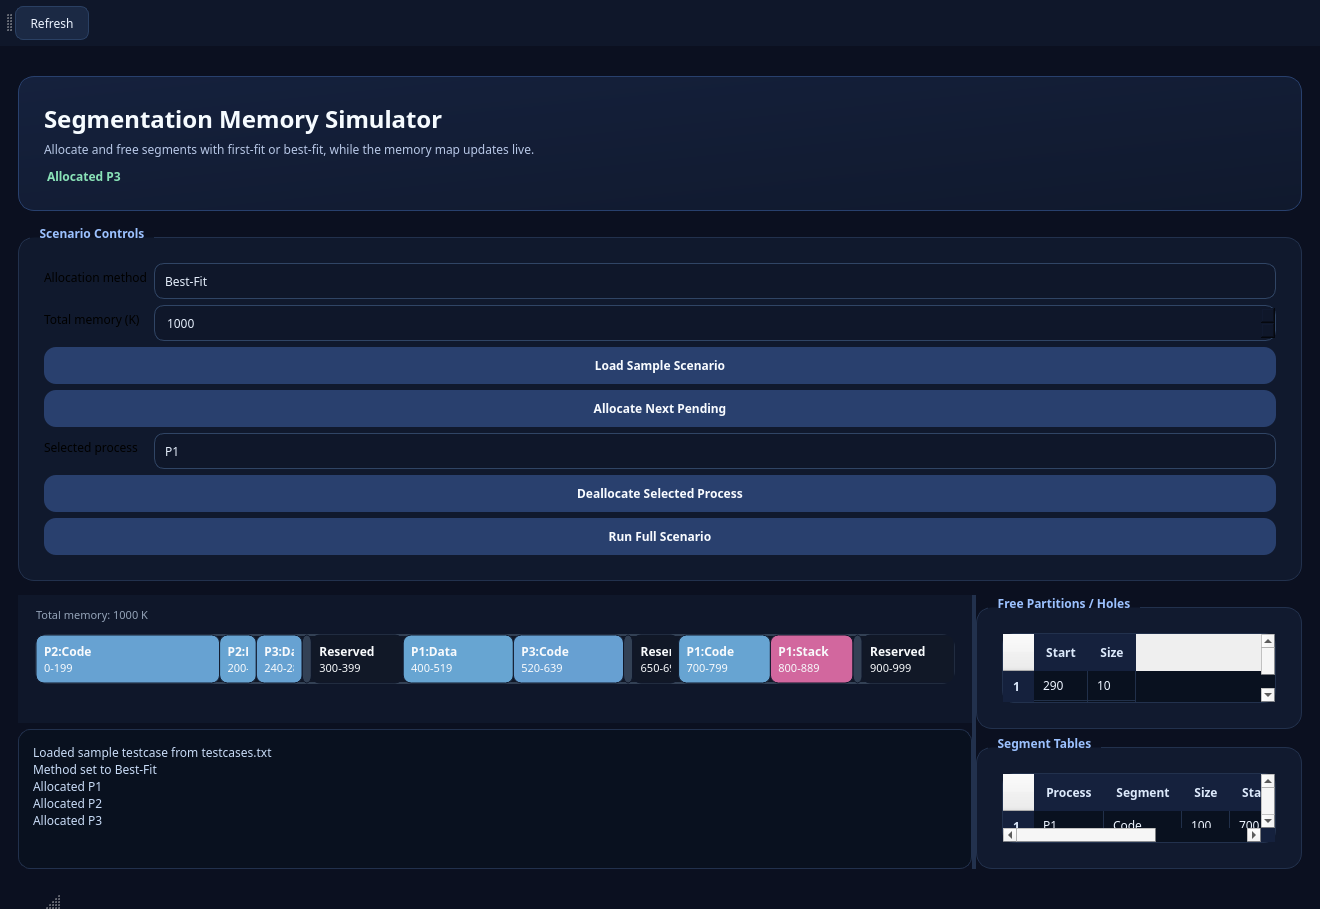
\includegraphics[width=\linewidth]{screenshots/bestfit/p3_attempted.png}
        \caption{P3 attempted}
    \end{subfigure}

    \vspace{0.5cm}

    \begin{subfigure}[t]{0.48\textwidth}
        \centering
        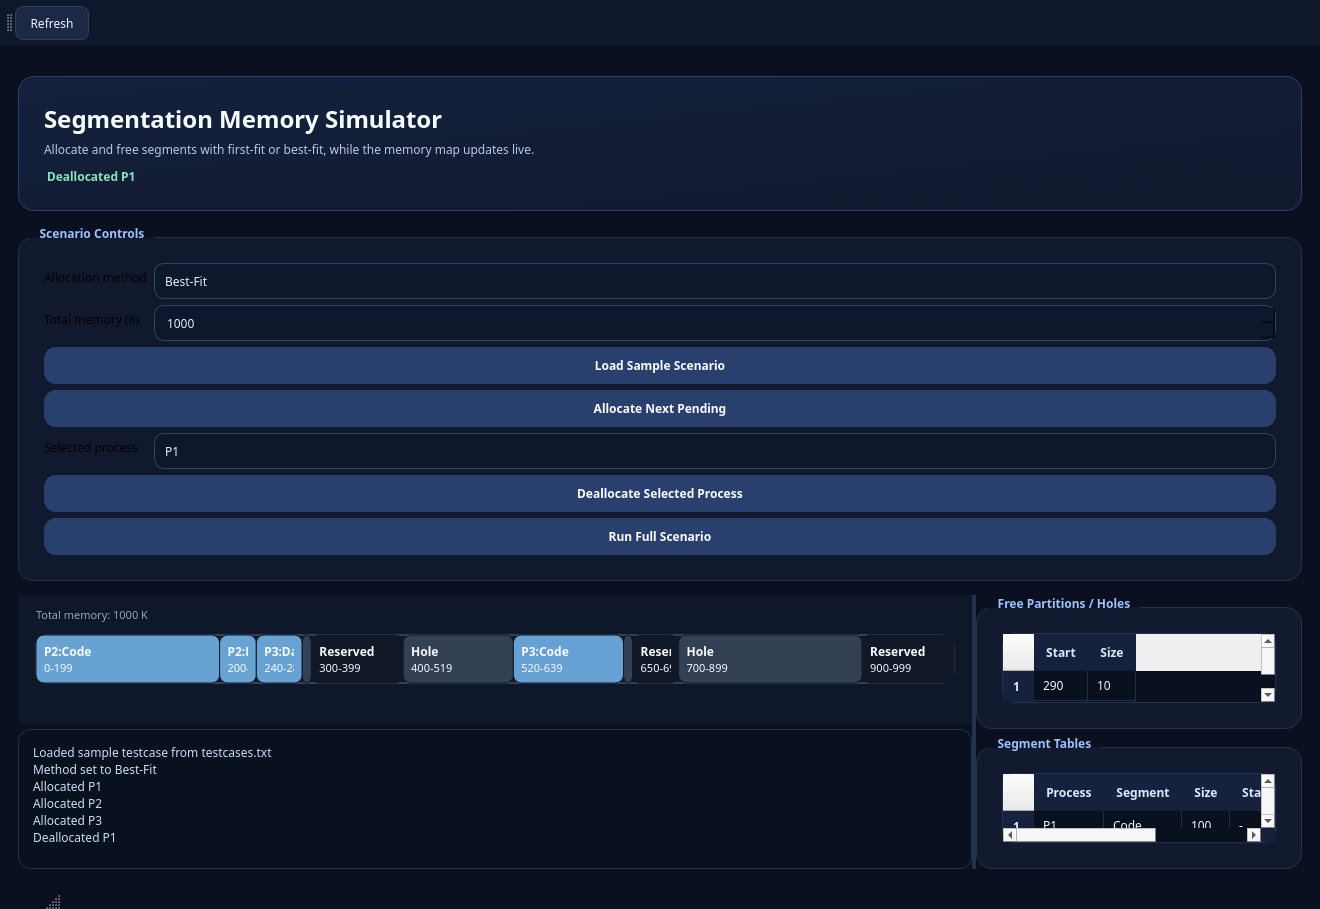
\includegraphics[width=\linewidth]{screenshots/bestfit/p1_deallocated.png}
        \caption{P1 deallocated}
    \end{subfigure}
    \hfill
    \begin{subfigure}[t]{0.48\textwidth}
        \centering
        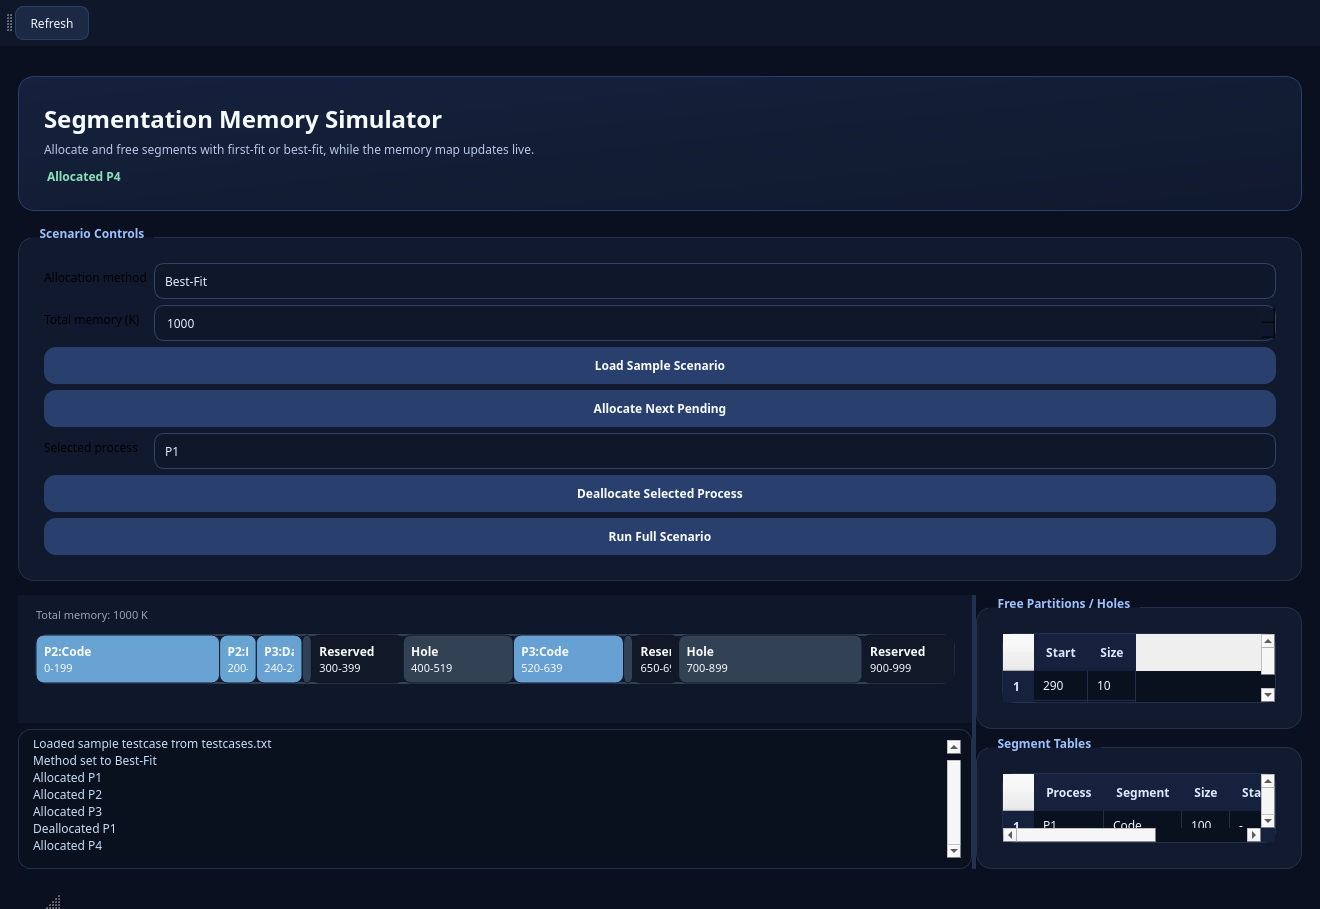
\includegraphics[width=\linewidth]{screenshots/bestfit/p4_allocated.png}
        \caption{P4 allocated}
    \end{subfigure}
    \caption{Best-Fit screenshots after each operation.}
\end{figure}

\section*{Short Comparison}
First-Fit chooses the first hole that fits, so it is faster. Best-Fit searches for the smallest suitable hole, so it usually reduces wasted space. The screenshots show how the two methods place the same processes differently.

\section*{Conclusion}
The project successfully shows segmentation-based allocation with a simple GUI and screenshot evidence for both algorithms.

\end{document}
